\documentclass[ms,electronic,letterpaper,lol,lof]{byumsphd}

\usepackage{amsmath}
\usepackage{graphicx}
\usepackage{listings}
%\usepackage[outputdir=build]{minted}
\usepackage{inconsolata}
\usepackage[T1]{fontenc}
\usepackage{natbib}
\usepackage{tikz}
\usetikzlibrary{positioning}
\usepackage{amsthm}
\usepackage{url}
\usepackage[toc]{appendix}

\newcommand{\racket}[1]{\mintinline{racket}{#1}}
% TODO: use natbib maybe?
\begin{document}

\title{Enabling Optimizations Through Demodularization} 

\author{Blake Johnson}

\committeechair{Eric Mercer}
\committeemembera{Christophe Giraud-Carrier}
\committeememberb{Quinn Snell}

\monthgraduated{December}
\yeargraduated{2015}
\yearcopyrighted{2015}

\documentabstract{%
Programmers want to write modular programs to increase maintainability and create abstractions, but modularity hampers optimizations, especially when modules are compiled separately or written in different languages. 
In languages with syntactic extension capabilities, each module in a program can be written in a separate language, and the module system must ensure that the modules interoperate correctly. 
In Racket, the module system ensures this by separating module code into phases for runtime and compile-time and allowing phased imports and exports inside modules. 
We present an algorithm, called demodularization, that combines all executable code from a phased modular program into a single module that can then be optimized as a whole program. 
The demodularized programs have the same behavior as their modular counterparts but are easier to optimize. 
We show that programs maintain their meaning through an operational semantics of the demodularization process and verify that performance increases by comparing modular Racket programs to the equivalent demodularized and optimized programs.
We use the existing Racket optimizer to optimize the demodularized programs by decompiling them into an intermediate form that the optimizer uses.
We also demonstrate a dead code elimination optimization that dramatically reduces the file size of demodularized Racket programs.
}


\documentkeywords{macros, Racket, modules, optimization}

\acknowledgments{%
I would like to thank Jay McCarthy for getting me interested in the field of programming languages, and for being both an advisor and mentor to me. I have enjoyed both our political and technical talks. Matthew Flatt has been an immense help in explaining to me the internals of the Racket runtime. He is always quick to respond to emails and offers salient solutions to problems I have had. I would also like to thank Eric Mercer, who took me on as his student after Jay left. I'm grateful for the opportunity he gave me to finish this thesis and the valuable input he gave in putting it together. Finally, I would like to thank my mom, Jane Johnson, for always believing in me and encouraging me to finish.
}%

\department{Computer~Science}
\graduatecoordinator{Quinn~Snell}
\collegedean{Thomas~W.~Sederberg}
\collegedeantitle{Associate~Dean}
\maketitle

\chapter{Introduction}
\label{chap:introduction}

Programmers should not have to sacrifice the software engineering goals of modular design and good abstractions for performance. 
Instead, their tools should make running a well-designed program as efficient as possible. 

Many programming languages provide features for creating modular programs. 
This may be as simple as separating code into different files or as complex as specifying separate interfaces and implementations for modules.
When code is separated into modules, it is possible to compile each module separately provided enough information is known about calls to other modules.
Separate compilation allows programmers to work on one part of their program without needing to recompile the whole program, but this convenience comes at a cost.
The compiler does not have much information about functionality from other modules as it compiles a single module, making optimizations more difficult.

A separately compiled program is turned into an executable through linking all of the modules together, which can happen either statically or dynamically.
Static linking creates a full executable program by combining all of the modules of the program before running the program.
Dynamic linking creates references to other modules in the program and loads them as needed when the program runs.
Linking is just one step in the process of taking a program from source code to running code, and programming languages oten have more steps that happen in that transformation process.

Some programming languages provide macro systems, which run before compiling, that enable programmers to add features to the programming language through manipulation of the syntax of the program.
Simple macro systems allow textual replacement, like the preprocessor in C/C++, while more advanced systems provide access to the syntax as objects with rich lexical information and a full programming language to manipulate the syntax.
Some of these more advanced macro systems even allow programmers to write macros in the same programming language they use to write their programs. 

These advanced macro systems give programmers the ability to extend a programming language in arbitrary ways, even to the point of being able to create domain specific languages as collections of macros.
When creating such programs, the details of individual macros are often hidden in modules, and, much like a separately compiled program, these modules need to be linked into an executable. 
Unlike a separately compiled program though, macros generate code, so they need to run before the program can be compiled.

Macros written in the same language as the program need to use the same compiler that the language uses, but the compilation needs to happen before normal program compilation.
Macros can also use other macros in their implementation, which means that those other macros must be ready to run (compiled) before their use.
This leads to an interleaving of compiling and running code that goes back and forth to ultimately produce the final program.

Separate compilation is more difficult in the presence of an advanced macro system.
Macros are defined side-by-side with program definitions, which means that macro definitions can be spread across modules and can also use functionality provided in separate modules.
A compiler for such a language must ensure that modular programs have the same meaning independent of the order in which the modules are compiled.

A solution to the problems of separate compilation with advanced macros is described by Flatt and implemented for the Racket programming language \cite{Flatt}.
He explains a method of compiling modules in phases, where each phase corresponds to which part of the program is running and which part of the program is compiling.
In this case, running means executing code, which includes executing macros, because macros are just code as well.
Compiling means translating code from source code to executable code, perhaps with macros doing part of the translation.
At phase 0, the main program is running and nothing is compiling.
At phase 1, the main program is compiling and macros that it uses are running.
At phase 2, the phase 1 macros are compiling and any macros used in the compilation of phase 1 macros are running, and so on.
The compiler starts compiling at the highest phase of the program (which can be upwards of phase 70 in normal Racket programs) and compiles each phase downward until it produces phase 0 code. 
By separating compilation into phases, it is possible to have a both a module system and a macro sytem coexist.

Separate compilation makes compiler optimization more difficult and less effective.
Good abstractions, provided by splitting a program into modules, are meant to obscure internal implementations so that it is easier for programmers to reason about their programs, but this obscurity also limits information available for optimizations. 
A single module compiled alone is difficult to optimize because the compiler has little to no information about values that come from other modules when compiling the module.
Existing optimizations have even less information when modules can extend the compiler, as modules can in languages with advanced macro systems. 

Language implementations have solved the problem of optimizing separately compiled programs in various ways.
Some implementations of languages avoid the problems associated with separate compilation by not allowing it. 
The whole-program optimizing compilers Stalin \cite{stalin} for Scheme and MLton \cite{mlton} for ML take this approach.
Other implementations do optmizations while statically linking the program.
There are options in gcc \cite{gcc} and clang \cite{clang} to do this type of optimization.
This type of optimization is usually done on machine code, so it can be too low level to do certain optimizations.
Some implementations perform cross-module inlining by selectively choosing functions to inline between modules.
Inlining must be heuristic-based, and good heuristics are hard to develop. 
Just-In-Time (JIT) compilers attack the problem in a different way by deferring optimizations until the program is running, where is has more information on the actual use of the program.

Our solution for optimizing modular programs in the presence of an advanced macro system, called demodularization, is to transform a modular program into a non-modular program by combining all runtime code and data in the program into a single module.
Conceptually, this is similar to what static linkers do in programming languages with separate compiliation.
After combining, the single module is then re-run through the existing optimizer, but this time the optimizer has information about the whole program.
This part is similar to doing link-time optimization for programming languages with separate compilation, but is at a higher level than most link-time optimizers.
Demodularization is meant to be done when producing the final production version of a program, so that during development, a programmer can still take advantage of separate compilation.

In a phased module system, finding all of the runtime values is not trivial.
Phased module systems allow programmers to refer to the same module while writing macros and while writing programs, but macros do not need to be included in the final program because they are only needed to compile the program.
In order to collect all of the code needed to run a modular program with phases, it is necessary to completely understand at what phases every module in the program is used. 
A demodularized program does not need to include modules that are only needed during compile-time, but whether or not the module is needed only at compile-time is not obvious from just examining the module in isolation. 

\paragraph{Thesis} Demodularizing programs in a language with a module system and an expressive macro system is feasible and yields more optimization opportunity for the compiler, resulting in more efficient code when compared to phased compilation and cross-module inlining.

We show that demodularization is feasible by implementing it for a simple language model and then implementing it for the Racket programming language.
We show that it is useful by showing that it maintains program meaning and that it improves performance and program size.

We explain the Racket module system in Chapter~\ref{chap:module-system}. In Chapter~\ref{chap:intuition}, we explain demodularization at a high level with a detailed example.
Next, we use the operational semantics model of the demodularization process to explain why demodularization is correct (Chapter~\ref{chap:model}), and we then describe an actual implementation for Racket (Chapter~\ref{chap:implementation}), followed by experimental results of demodularizing and optimizing real-world Racket programs (Chapter~\ref{chap:evaluation}). 
The operational semantics model removes the unnecessary details of the full implementation so the demodularization process is easier to understand and verify. 
The actual implementation presents interesting difficulties that the model does not.
The experimental results show that demodularization improves performance, especially when a program is highly modular. 

\chapter{The Racket Module and Macro Systems}
\label{chap:module-system}

Demodularization is made to run on a program written in a language that combines macros and modules.
For this research, we chose to implement demodularization for the Racket programming language because of its advanced macro and module systems.
This chapter gives background information on Racket through a detailed example program that demonstrates macro and module usage.

% DONE: rewrite this section
\section{The Racket Programming Language}
The Racket Programming Language is a platform for creating powerful abstractions.
These abstractions are created through the use of Racket's macro and module systems. 
The macro system, a heritage from LISP~\cite{LISP} and Scheme~\cite{scheme}, allows programmers to add new features to their programs in an integrated way.
The module system allows programmers to separate their programs into logical parts and hide implementation details. 
Together, they allow programmers to create Languages as Libraries~\cite{lal} that are suitable for specific tasks.

% TODO: mention that programs can extend themselves in the same file
\section{Macros}
Macros are the main way programmers add new features to Racket. 
Macros are written alongside normal functions in a program, but they are used during the compilation of the program. 
Essentially, macros are functions (known as transformers) whose domain and range are syntax objects.
Syntax objects are data structures that contain the raw syntax of a program, along with lexical information and other properties associated with the syntax.
If a programmer needs the power, they can write transformers using all of the features of Racket, as long as the function takes in and produces syntax objects.
Racket provides pattern-matching for syntax objects that makes writing macros simpler when that is all that a programmer needs.

The \racket{define-syntax} form is used to identify a macro definition that is a function from syntax to syntax.
The helper function, \racket{syntax-case} matches syntax patterns so that it is easy to use them in the output of the macro.

% DONE: example should use a function or letrec, not let loop
% DONE: maybe just use syntax-case here
\begin{listing}[tb]
  \inputminted{racket}{listings/while-macro.rkt}
  \caption{a macro implementation of a \racket{while} loop}
  \label{lst:while-macro.rkt}
\end{listing}
Listing~\ref{lst:while-macro.rkt} shows how to use one of these macros to write a \racket{while} loop. 
The macro turns a \racket{while} loop into a recursive function and a call to that recursive function.
Whatever syntax used by the programmer for the \racket{test} and \racket{body ...} forms will be substituted by \racket{syntax-case} into the output of the macro. 
Listing~\ref{lst:while-expanded.rkt} shows a use of the while macro and what it expands into after running the macro. 
\begin{listing}[tb]
  \inputminted{racket}{listings/while-expanded.rkt}
  \caption{use and expansion of a \racket{while} loop}
  \label{lst:while-expanded.rkt}
\end{listing}
% DONE: example expansion
% DONE: fuller explanation of hygeine with citation
Racket's macros are hygienic \cite{hygiene}, which means that identifiers created from programs will not clash with identifiers created from macros. 
This means that macros are protected from the surrounding program changing their identifiers, and also that the program is protected from the macro changing its identifiers.
In this example that means that the Racket program using a while loop will not be able to call the \racket{while-loop} function that the macro creates, and that if the program has another definition for \racket{while-loop}, it will be independent from the definition introduced by the macro.
Also, each use of the macro will have distinct definitions for \racket{while-loop} so that the macro can be nested and used multiple times.
\section{Modules}
% TODO: all listings are modules in separate files
Racket modules are a way of grouping definitions, expressions, and macros. 
Modules also allow control over imports and exports, using the Racket forms \racket{require} and \racket{provide} respectively.
Listing~\ref{lst:counter.rkt} shows a simple Racket module and some of the features of the Racket module system.
\begin{listing}[tb]
  \inputminted{racket}{listings/counter.rkt}
  \caption{\texttt{counter.rkt}: A simple Racket module implementing a counter}
  \label{lst:counter.rkt}
\end{listing}
The \texttt{counter} module contains a variable definition and functions for getting and incrementing that variable.
The module only exports the functions, so the module encapsulates the variable.
If a programmer wanted to use this module, they would import it using \racket{require} as shown in Listing~\ref{lst:while-test.rkt}. 

\begin{listing}[tb]
  \inputminted{racket}{listings/while-test.rkt}
  \caption{\texttt{while-test.rkt}: A Racket module that uses other modules}
  \label{lst:while-test.rkt}
\end{listing}

It is also possible to use modules to help write macros.
For example, if a programmer wanted to change the \racket{while} macro so that it reported how many expressions were in each while loop, they could use the \texttt{counter} module inside the \racket{while} definition as seen in Listing~\ref{lst:while-lang.rkt}.
\begin{listing}[tb]
  \inputminted{racket}{listings/while-lang.rkt}
  \caption{\texttt{while-lang.rkt}: A Racket module implementing a language with \racket{while} loops}
  \label{lst:while-lang.rkt}
\end{listing}
It is possible to add code to the \racket{while} macro because it is just a function from syntax to syntax that runs at compile-time. 
Also, the \racket{require} form includes a \racket{for-syntax} form to indicate that the \texttt{counter} module is needed at compile-time (along with the \racket{racket/base} module for \racket{printf}).
Now this module can be used to extend the language of other programs by adding a \racket{while} loop, although it is just a library that is included like any other library.

\section{Languages}
% TODO: Rewrite this section, it sucks
The ability to use modules as languages allows programmers to write specialized domain-specific languages (DSLs) to better express solutions to domain problems. 
% TODO: akward sentence
Using this ability, programmers have added languages for Typed Racket~\cite{typed}, Object-Oriented Racket~\cite{oo}, Logic Programming~\cite{logic}, and more.
Also, because they are modules, it is possible to use them all in the same program and use the right language for each specific problem.
The language creating facilities of Racket extend to more than just collections of functions and macros; they also allow changing the parser and changing the meaning of things like function application syntax. 

\section{Separate Compilation}
In the presence of macros that can run arbitrary code, compilation of a single module becomes complicated. 
Compilation and execution of code has to be interleaved in order to produce the correct compiled program.
% DONE: explain that listings form a program with multiple modules and while-test is main
% DONE: include module dependency figure
All of the listings in the previous section form a program with the \racket{while-test} module as the main module.
Figure~\ref{fig:modules.tex} shows the relationship between the different modules in the program.
\begin{figure}
  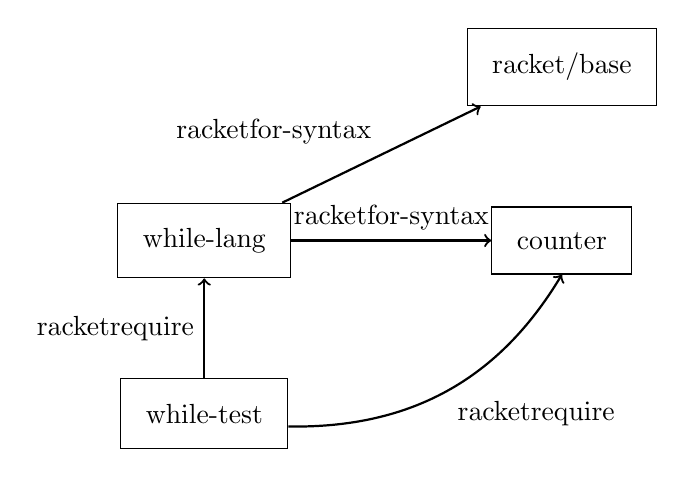
\begin{tikzpicture}
  [node distance=.5in and 1in,
   module/.style={rectangle,draw,inner sep=.125in}
  ]
\node (obj-run)    [module]  {counter};
\node (racket-base) [module] [above=of obj-run] {racket/base};
\node (while-lang) [module] [left=of obj-run] {while-lang}
  edge [->, thick] node[auto]{\racket{for-syntax}} (obj-run)
  edge [->, thick] node[auto]{\racket{for-syntax}} (racket-base);
\node (while-test) [module] [below=of while-lang] {while-test}
  edge [->, thick] node[auto]{\racket{require}} (while-lang) 
  edge [->, thick, bend right] node[swap,auto]{\racket{require}} (obj-run.south);
\end{tikzpicture}

  \caption{Module dependencies for the \racket{while-test} program}
  \label{fig:modules.tex}
\end{figure}
To compile the program, both the \racket{while-lang} and \racket{counter} need to be compiled before \racket{while-test}, but also the \racket{counter} module needs to be compiled and ready to use while compiling \racket{while-test} because the counter functions are used inside the \racket{while} macro.
While compiling \racket{while-test}, the \racket{while} macro will be expanded and code from the \racket{counter} module will run.
The value of the counter is not shared between compiling \racket{while-test} and running it.

\section{Phases}
The way the Racket module system allows for reliable separate compilation is by separating compilation and execution into phases.
Phase 0 is the execution phase of the main module of a program, what could be considered running the program.
Phase 1 is the compilation phase of the main module, which could include execution of code inside macros. 
A module can contain both phase 0 and phase 1 code; regular function definitions are phase 0, and macro definitions are phase 1.

Higher phases occur when macros use other macros in their implementation.
Another way higher phases occur is by importing modules for use inside a macro.
In the example program, the \racket{while-lang} module imports the \racket{counter} module using \racket{for-syntax}.
The \racket{for-syntax} form means that the module will be included for use at phase 1 relative to the including module, so that its code is available to use inside macro definitions.
There is an analogous form, \racket{for-template}, that will include code at phase -1 relative to the including module, so that the included module's code will be available for use inside the output of a macro. 
By allowing references to relative phases going in both directions, a Racket program can have a complex structure of imports and exports.

It is possible for a single module to be used in multiple phases, and each phase will have a separate instantiation of the module.
In the example program above, the \racket{counter} module will be instantiated twice, once for use while macros are running at phase 1, and once for use while the main program is running at phase 0.

Even though compilation of a program can go through many phases and interleave compiling and running code many times, side effects that occur during this process are discarded. 
The separate compilation guarantee of the Racket module system is that ``Any effects of the instantiation of the module's phase 1 due to compilation on the Racket runtime system are discarded'' \cite{sep}. 

\section{Program Evaluation}
Running a separately compiled Racket program involves following all of the \racket{require} forms and running all phase 0 code in the order in which the code is imported.
It is possible that there will be phase 0 code to run from an imported module where the import path to that module includes phase shifts.
Module phases are relative to one another, so if one module imports a module at phase 1, which then imports a different module at phase -1, the code in the third module will be at phase 0 relative to the first module and must be run in the final program.

By understanding how Racket programs are compiled and evaluated, it is apparent that only phase 0 code is necessary to run the program. 
This is the basis for how demodularization can recover whole programs from separately compiled Racket modules. 

\chapter{Intuition}

Demodularization enables whole-program optimizations and eliminates module loading overhead while maintaining the runtime meaning of a program.
To understand how demodularization preserves the runtime meaning of a program, we first need to understand the runtime meaning of a modular Racket program.
Consider the program in Figure~\ref{main-rkt}.

\begin{figure}[h]
\begin{schemedisplay}
#lang racket/base
(require "queue.rkt")

(with-queue (1 2 3 4 5 6)
  (enqueue 4)
  (displayln (dequeue))
  (displayln (dequeue)))
\end{schemedisplay}
\caption{\texttt{main.rkt}}
\label{main-rkt}
\end{figure}

This program imports a queue library through a \scheme{require} expression and then uses the library to do some queue operations.
Figures~\ref{queue-rkt},~\ref{long-queue-rkt}, and~\ref{short-queue-rkt} contain the three modules that make up the queue library.
The library consists of a macro and two queue implementations, where the macro decides which implementation to use based on the length of the initial queue at compile time.

\begin{figure}[h]
\begin{schemedisplay}
#lang racket/base
(require (for-syntax racket/base
                     racket/syntax)
         "short-queue.rkt"
         "long-queue.rkt")

(define-syntax (with-queue stx)
  (syntax-case stx ()
    [(with-queue (v ...) e ...)
     (begin
       (define type 
         (if (> (length (syntax->list #'(v ...))) 5) 
	     'long 
             'short))
       (define make-queue 
         (format-id #'stx "make-~a-queue" type))
       (define enqueue (format-id #'stx "~a-enqueue" type))
       (define dequeue (format-id #'stx "~a-dequeue" type))
       #`(let ([q (#,make-queue v ...)])
           (define (#,(datum->syntax stx 'dequeue)) 
             (#,dequeue q))
           (define (#,(datum->syntax stx 'enqueue) x)
             (#,enqueue q x))
           e ...))]))

(provide with-queue)
\end{schemedisplay} 

\caption{\texttt{queue.rkt}}
\label{queue-rkt}
\end{figure}

\begin{figure}[h]
\begin{schemedisplay}
#lang racket/base
(define (make-long-queue . vs)
  .... make-vector ....)

(define (long-enqueue q v)
  .... vector-set! ....)

(define (long-dequeue q)
  .... vector-ref ....)

(provide (all-defined-out))
\end{schemedisplay}
\caption{\texttt{long-queue.rkt}}
\label{long-queue-rkt}
\end{figure}

\begin{figure}[h]
\begin{schemedisplay}
#lang racket/base
(define (make-short-queue . vs)
  .... list ....)

(define (short-enqueue q v)
  .... cons ....)

(define (short-dequeue q)
  .... list-ref ....)

(provide (all-defined-out))
\end{schemedisplay}
\caption{\texttt{short-queue.rkt}}
\label{short-queue-rkt}
\end{figure}

The Racket runtime evaluates this program by compiling and then running the main module.
Whenever the runtime encounters a \scheme{require} expression during compilation, it either loads an existing compiled version of the required module or compiles the required module.
Whenever the runtime encounters a macro expression during compilation, it expands the macro.
In this example, the runtime begins to compile \texttt{main.rkt} and loads the compiled version of \scheme{racket/base}. 
Next, it encounters the \scheme{require} expression for \texttt{queue.rkt} and compiles it.
Compilation of \texttt{queue.rkt} triggers compilation of both \texttt{short-queue.rkt} and \texttt{long-queue.rkt}. 

After finishing \texttt{queue.rkt}, the runtime returns to \texttt{main.rkt} and expands the \scheme{with-queue} macro.
The \scheme{with-queue} macro checks the length of the initial queue, which in this case is six, and chooses to use the \scheme{long-queue} implementation.
The macro expands into a \scheme{let} expression that binds the identifier \scheme{q} to the initial queue, along with internal definitions of \scheme{enqueue} and \scheme{dequeue} that use the \scheme{long-queue} implementations.
Figure~\ref{main-expanded-rkt} shows what \texttt{main.rkt} looks like after expansion.

\begin{figure}[h]
\begin{schemedisplay}
(module main racket/base
  (#%module-begin
   (require "queue.rkt")
   (let ((q (make-long-queue 1 2 3 4 5 6)))
     (define (dequeue) (long-dequeue q))
     (define (enqueue x) (long-enqueue q x))
     (enqueue 4)
     (displayln (dequeue))
     (displayln (dequeue)))))
\end{schemedisplay}
\caption{\texttt{main.rkt} expanded}
\label{main-expanded-rkt}
\end{figure}


After compiling the whole program, the Racket runtime evaluates the program by loading and executing the compiled main module.
As is the case with compilation, evaluation also follows the \scheme{require} expressions and runs required modules as it encounters them.
In this example, the runtime evaluates \texttt{main.rkt} and encounters the \scheme{require} expression for \texttt{queue.rkt}.
It then follows the \scheme{require}s for \texttt{short-queue.rkt} and \texttt{long-queue.rkt} and installs the definitions that those modules provide.
When evaluation returns to \texttt{queue.rkt}, nothing else happens because macros are only needed at compile time.
Finally, evaluation returns to \texttt{main.rkt} and the runtime evaluates the rest of the program.

A demodularized version of this program should contain all code that ran while evaluating the modular program, minus the module loading steps.
The demodularization algorithm starts with the compiled versions of all of the modules for the program, and then traces the \scheme{require} expressions and includes all runtime code into a single module in the order it encounters the code.
Figure~\ref{main-demod-rkt} shows what the single module looks like after running the demodularization algorithm on it.
There are no require statements and the macro definition is gone, but the all the code that ran during the evaluation of the modular version is there in the same order as before.

\begin{figure}[h]
\begin{schemedisplay}
(module main racket/base
  (#%module-begin
   (define (make-short-queue . vs)
    .... list ....)

   (define (short-enqueue q v)
    .... cons ....)

   (define (short-dequeue q)
    .... list-ref ....)

   (define (make-long-queue . vs)
    .... make-vector ....)

   (define (long-enqueue q v)
    .... vector-set! ....)

   (define (long-dequeue q)
    .... vector-ref ....)

   (let ((q (make-long-queue 1 2 3 4 5 6)))
     (define (dequeue) (long-dequeue q))
     (define (enqueue x) (long-enqueue q x))
     (enqueue 4)
     (displayln (dequeue))
     (displayln (dequeue)))))
\end{schemedisplay}
\caption{\texttt{main.rkt} demodularized}
\label{main-demod-rkt}
\end{figure}


This example is rather simple because it only uses a single macro, but in practice, Racket programs use many macros, even macros that use other macros in their implementations, creating a language tower.
The demodularization algorithm takes this into account by only gathering runtime code while tracing through \scheme{require} expressions.
The details about how this works is further explained in the operational semantics model in Chapter 3.

With all of the code in a single module, it is easy to see how standard optimizations such as inlining and dead code elminiation can reduce the module to the code in Figure~\ref{main-demod-opt-rkt}.
\begin{figure}[h]
\begin{schemedisplay}
(module main racket/base
  (#%module-begin
   (let ((q (.... make-vector .... 1 2 3 4 5 6 ....)))
     (.... vector-set .... 4 ....)
     (displayln (.... vector-ref ....))
     (displayln (.... vector-ref ....)))))
\end{schemedisplay}
\caption{\texttt{main.rkt} demodularized and optimized}
\label{main-demod-opt-rkt}
\end{figure}
In this simple example, with constant folding this progam could be optimized even more, but even in programs with dynamic inputs, demodularization enables many optimizations that aren't possible when the program is separated into modules.


\chapter{Model}

We can understand the specifics of demodularization by describing it as an algorithm for a simple language with a well defined semantics.
The \emph{mod} language (Figure~\ref{source-lang}) contains only the features necessary to write modular programs where it is possible to observe the effects of module evaluation order.

\begin{figure}[h]
\includegraphics{source}
\caption{\emph{mod} language grammar}
\label{source-lang}
\end{figure}

A program in \emph{mod} consists of a list of modules that can refer to each other.
Each module has a name, any number of imports, any number of definitions, and sequenced code expressions. 
All definitions in a module are exposed as exports to other modules, but to use definitions from another module, the program must import it through a \scheme{require} expression.
Both \scheme{require} and \scheme{define} expressions have phase annotations; this simulates the interactions between modules in a language with macros and a language tower without requiring a model of macro expansion.
The language includes variable references, numbers, addition, and mutation.
Mutation makes module evaluation order observable, and addition represents the work that a module does.
In addition to numbers and variables, there are two special forms of values and references that model the interaction of macros with the module system.
A \scheme{quote} expression is like a reference to syntax at runtime.
A \scheme{ref} expression is like a macro that can only do one thing: refer to a variable at a phase.

The \emph{mod} language exposes phases as an integral part of the language, while languages like Racket keep phases obscured from the end user even though it uses phases during compiling and evaluating a program.
So, what is a phase?
In the discussion of the example program in section XXX, we used the terminology of runtime and compile-time.
Phases are just numerical designations for these terms, where runtime is phase 0 and compile-time is phase 1.
The reason phases are numbers is because phases exist outside of the range of 0 to 1.
Given that phase 1 is the compile-time for phase 0, we can extend this idea so that phase 2 is the compile-time for phase 1.
Conversely, compile-time code generates code for the phase below it, so it can refer to bindings at negative phases.
(Talk about relative phases)
Phases allow programmers to build syntactic abstractions that use other syntactic abstractions, creating a tower of intermediate languages.
The \emph{mod} language does not allow programmers to create language towers, but evaluating a \emph{mod} program uses the same mechanisms as evaluating a Racket program.

We have to compile \emph{mod} programs before demodularizing them, just like in the Racket implementation.
In Racket, compiling expands all macros in a program and changes definitions and variable references to refer to memory locations.
In \emph{mod}, compiling eliminates \scheme{ref} expressions, turns definitions into \scheme{set!} expressions, changes variable references to include module information, and sorts code into phases.
Compilation in both cases still leaves behind a relatively high-level language, but the language is free of syntactic extensions.
This is important for demodularization because otherwise macro expansion would have to be part of the algorithm, which would complicate it and possibly duplicate work.
The grammar in Figure~\ref{compiled-lang} specifies the compiled language for \emph{mod}.

\begin{figure}[h]
\includegraphics{compiled-lang}
\caption{compiled language grammar}
\label{compiled-lang}
\end{figure}

We evaluate the compiled language using a small-step reduction semantics. 
Because the reduction rules are syntactic, we extend the compiled language further with evaluation contexts, a heap representation, and a stack representation to keep track of the order to instantiate modules.
These extensions are in Figure~\ref{compiled-eval-lang}.
An expression of the form:
\setspecialsymbol{sigma}{$\sigma$}
\begin{schemedisplay}
(sigma / (mod ...) / ((id phase) ...)  / ((id phase) ...))
\end{schemedisplay}
represents the state of the machine during evaluation.
$\sigma$ represents the heap of the program, and when evaluation finishes represents the output of the program.
The list of modules is the code of program in the compiled language.
The first list of \scheme{(id phase)} pairs is the list of modules to evaluate, and the second list is the modules that have already been evaluated.

\begin{figure}[h]
\includegraphics{compiled-eval-lang}
\caption{extensions to compiled language grammar}
\label{compiled-eval-lang}
\end{figure}

The reduction rules in Figure~\ref{eval-reduction} evaluate a compiled program that starts with an empty heap, the program code, a stack that contains the identifier of the main module at phase 0, and an empty completed module list. 

\begin{figure}[h]
\includegraphics[width=\textwidth]{eval-reduction}
\caption{modular evaluation}
\label{eval-reduction}
\end{figure}

The \emph{module require} rule matches a program with a \scheme{require} expression in the module at the top of the evaluation stack and evaluates it by removing the \scheme{require} expression from the module and pushing the required module onto the evaluation stack with the phase shifted appropriately.
The current module is still on the stack and will continue evaluating after the required module is done evaluating.
The subsequent rules all apply only when the phase relative to the main module is zero.
The \emph{var ref} rule looks up a variable in the heap and replaces the variable with its current value.
The \emph{add} rule replaces an addition expression of numbers with the result of computing their sum.
The \emph{set!} rule installs a value for a variable into the heap and reduces to the value.
When an expression is a value, the \emph{expression done} rule matches and removes the expression from the module.
When there are no more expressions left in a module, the \emph{module done} rule applies by removing the module from the program and placing a reference to it in the list of finished modules.
The \emph{module done already} rule applies when the current module on the stack is in the finished list, so that modules are not evaluated multiple times. 

Figure~\ref{demod-redex} shows the demodularization algorithm for the compiled language.
\begin{figure}[h]
\includegraphics[width=\textwidth]{demod-redex}
\caption{Demodularization algorithm}
\label{demod-redex}
\end{figure}


\chapter{Implementation}
\label{chap:implementation}

The implementation of demodularization for the Racket module system integrates with the existing compilation process. 
The goal of the implementation was to write the actual algorithm in Racket, but to use as much of the existing infrastructure as possible. 
We did not want to duplicate work done by the compiler, so the demodularization algorithm operates on Racket bytecode. 
We also did not want to duplicate work done by the optimizer, so we pass the demodularized program through the existing optimizer.
All of the pieces of the demodularization process are contained within a command line tool. 

\section{Racket Compilation Process}

Figure~\ref{fig:compilation} shows the compilation process that a Racket module undergoes and the various intermediate forms the code takes.
\begin{figure}
  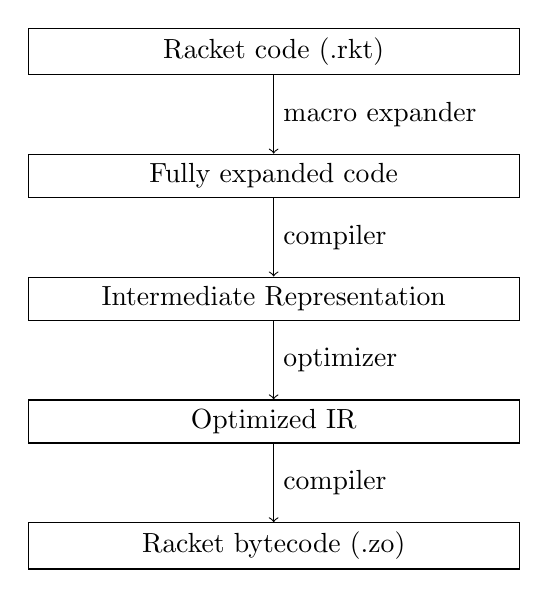
\begin{tikzpicture}[rep/.style={draw, text width=6cm, align=center}]
  \node (racket) [rep] {Racket code (.rkt)};
  \node (expanded) [rep, below=of racket] {Fully expanded code};
  \node (IR) [rep, below=of expanded] {Intermediate Representation};
  \node (OIR) [rep, below=of IR] {Optimized IR};
  \node (zo) [rep, below=of OIR] {Racket bytecode (.zo)};

  \draw[->] (racket)--(expanded) node [midway, right] {macro expander};
  \draw[->] (expanded)--(IR) node [midway, right] {compiler};
  \draw[->] (IR)--(OIR) node [midway, right] {optimizer};
  \draw[->] (OIR)--(zo) node [midway, right] {compiler};

\end{tikzpicture}

  \label{fig:compilation}
  \caption{Racket compilation process}
\end{figure}
In principle it would be possible to write the demodularization algorithm for modules at any point in this process, but we chose to write it at the bytecode level because it is a well defined file type and phases are clearly deliniated.

The compilation process for Racket is all written in C.
The first step of compiling a Racket module is to expand all of the macros it uses into what is known as the Racket kernel language or fully expanded code.
The next step is compilation to an Intermediate Representation (IR) made up of C data structures.
The optimizer works on this IR to produce an optmized version of it.
Then, the compiler finishes turning the IR into bytecode.

\section{Racket bytecode}
Racket bytecode is different from most other forms of bytecode in that it mostly maintains the structure of the abstract syntax tree from the original program.
The main aspect that changes between fully-expanded Racket programs and Racket bytecode is the use of stack positions instead of variables and the addition of stack-manipulating instructions.
A full explanation of Racket bytecode and what it means can be found in "The Racket virtual machine and randomized testing" \cite{bytecode}.

% DONE: Don't start a paragraph with Also
A table is created in the bytecode for the top level bindings in a module, which is known as the prefix.
All top level bindings have an entry in the prefix, including bindings that come from other modules, and any use of a top level binding in a program is replaced with a numeric reference to the entry.
Listing~\ref{lst:kernel.rkt} shows a simple program written in the most basic language that Racket supports: the \racket{kernel} language.
\begin{listing}
  \inputminted{racket}{listings/kernel.rkt}
  \caption{Example program written in \racket{kernel} language}
  \label{lst:kernel.rkt}
\end{listing}
When this code is compiled, it turns into the bytecode in Listing~\ref{lst:kernel-bytecode.rkt}. 
\begin{listing}
  \inputminted{racket}{listings/kernel-bytecode.rkt}
  \caption{Bytecode representation of program from Listing~\ref{lst:kernel.rkt}}
  \label{lst:kernel-bytecode.rkt}
\end{listing}

% DONE: comment on primval
In the bytecode, all references to the variable \racket{y} have been replaced with references to the prefix in the form of \racket{(toplevel 0)}. 
All references to \racket{displayln} have also been replaced with \racket{(toplevel 1)} references, which in turn references element \racket{7} of the prefix of the \racket{racket/private/misc} module.
The references to \racket{x} are now all different because the stack changes between each usage of \racket{x}.
The references to \racket{random} and \racket{+} are replaced with references to primitive implementations in the Racket runtime. 

\section{Demodularization}

The implementation of demodularization for the Racket module system is written in Racket and consumes and produces Racket bytecode.
Figure~\ref{fig:demod} shows the demodularization process and how it interacts with existing Racket components.
The library for reading and writing Racket bytecode in Racket was mainly used for debugging purposes and was incomplete, so the first task was to fully implement the Racket bytecode library.
\begin{figure}
  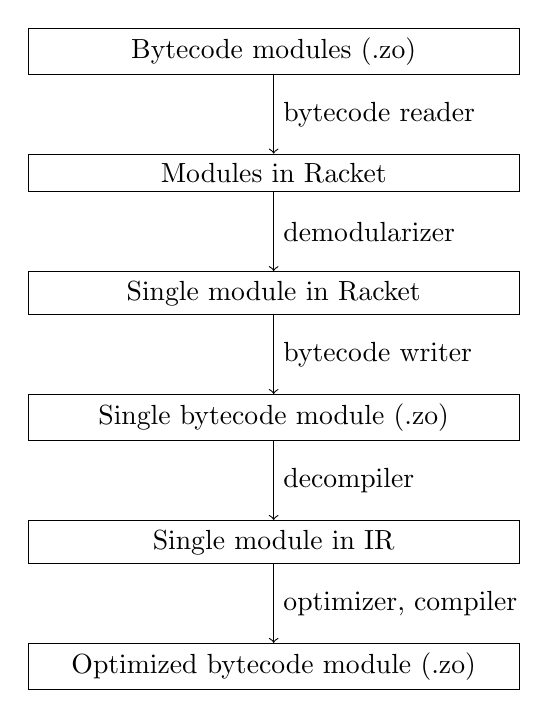
\begin{tikzpicture}[rep/.style={draw, text width=6cm, align=center}]
  \node (modules) [rep] {Bytecode modules (.zo)};
  \node (racket) [rep, below=of modules] {Modules in Racket};
  \node (demod) [rep, below=of racket] {Single module in Racket};
  \node (demod-zo) [rep, below=of demod] {Single bytecode module (.zo)};
  \node (IR) [rep, below=of demod-zo] {Single module in IR};
  \node (opt-zo) [rep, below=of IR] {Optimized bytecode module (.zo)};

  \draw[->] (modules)--(racket) node [midway, right] {bytecode reader};
  \draw[->] (racket)--(demod) node [midway, right] {demodularizer};
  \draw[->] (demod)--(demod-zo) node [midway, right] {bytecode writer};
  \draw[->] (demod-zo)--(IR) node [midway, right] {decompiler};
  \draw[->] (IR)--(opt-zo) node [midway, right] {optimizer, compiler};
\end{tikzpicture}

  \label{fig:demod}
  \caption{Demodularization process}
\end{figure}

The actual algorithm for demodularization is similar to the model in the previous chapter in that it traces requires and includes all phase 0 code in the final module, but it also has to deal with the module prefix and references to the prefix.
When the algorithm includes a required module, it also includes that module's prefix appended to the end of the main module's prefix. 
Then, it must adjust all references in that module's code to point at the new combined prefix.
Also, the algorithm tracks cross-module references and rewrites them to point to the new prefix as well.
In the example in Listing~\ref{lst:kernel-bytecode.rkt}, when the algorithm includes the module \racket{racket/private/misc} it must rewrite the reference to \racket{(toplevel 1)} to whatever the new position for \racket{displayln} is in the combined prefix.
% TODO: show a demod example

\section{Optimization}

For demodularization to be useful, the program needs to be optimized after demodularizing it.
% TODO: relate back to thesis rather than say we wanted
To optmize the demodularized bytecode, we wanted the existing Racket optimizer built into the Racket compiler so that we get all existing optimizations ``for free'' and any new optimizations in the future will work on both regularly compiled and demodularized programs.
The existing optimizer works on an intermediate form between fully-expanded Racket code and Racket bytecode.
This intermediate form only exists as C data structures in the implementation of Racket.
Therefore, to use the existing optimizer, Racket bytecode needed to be decompiled into this intermediate form. 

\section{Decompilation}

The decompiler was written in C, so that it could interoperate with the optimizer.
There are three main differences between Racket bytecode and the intermediate form: stack positions, cyclic closures, and reference arguments.
In Racket bytecode and in the intermediate form, all references to bindings are numeric, but in bytecode the references are stack positions and in the intermediate form the references are lexical.
For example, the bytecode in Listing~\ref{lst:kernel-bytecode.rkt} has three references to \racket{x}, in the form of \racket{(install-value 0 5)}, \racket{(local 1)}, and \racket{(local 3)}. 
% DONE: explain why they should all be 0
In the intermediate form, all of these references to \racket{x} should be \racket{0} because lexically they all refer to the same variable that is the closest binding.

Racket bytecode allows for cyclic closures, or closures which contain a reference to themselves.
Nothing like this exists in the intermediate form, so to decompile cyclic closures, the decompiler creates a new top level definition for the closure and replaces references to the closure (including the self-references) with references to the top level definition.
% TODO: maybe an example of this as well

Finally, Racket bytecode allows reference arguments (like C++ reference arguments) in functions, but the intermediate form doesn't allow them.
The decompiler turns reference arguments into \racket{case-lamdba} closures over the reference arguments with one case for getting the argument value and one case for setting the argument value. 

% TODO: how to know if it works (verification) paragraph
The decompilation algorithm is not the identity function when composed with compilation because of the transformations performed on cyclic closures and reference arguments.
Sometimes the optimizer will remove the \racket{case-lambda} arguments and turn them back into reference arguments, but this is not guaranteed. 
Racket has robust bytecode verification built in to the module loading system, so errors that were introduced by the decompiler were mostly caught by bytecode verification.

\section{Limitations}

Racket provides features that treat modules as first-class objects during runtime. 
For example, programs can load and evaluate modules at runtime through \racket{dynamic-require}. 
Because the demodularizer cannot know ahead of time what modules might be loaded at runtime, it disallows programs that use \racket{dynamic-require}.
If the modules loaded through \racket{dynamic-require} were completely separate (meaning they do not share any required modules) from the main program, it would be possible to demodularize the program, but in practice most modules required at runtime will share with the main program.

The restriction of not allowing \racket{dynamic-require} means that programs that need to load modules on the fly, such as REPLs, sandboxed evaluation environments, and scripting environments cannot be demodularized.
This is okay because such programs are fundamentally incomplete programs whose full meaning isn't known until runtime.

\section{Usage}
The implementation of demodularization is included in the Racket distribution as part of the build tool \racket{raco}. 
Users can pass in a module they would like to demodularize and optmize to the tool and it will compile all the necessary modules, run the demodularization algorithm on them, decompile the resulting module, and run optimizations on it to produce the final module.
For example, to demodularize a program whose main module was \texttt{while-test.rkt}, a user would type the following command: 

\begin{verbatim}
raco demod -O while-test.rkt
\end{verbatim}


\chapter{Evaluation}
\label{chap:evaluation}

For demodularization to be useful, it should improve performance of modular programs.
To test whether or not this is the case, we created benchmarks to test the speed of demodularized programs versus their modular counterparts.
We also compare the results with the cross-module inliner included in Racket.
We show improvements in the size of programs through the use of a dead-code elimination algorithm.
Finally, we discuss further improvements that demodularization can enable.

\section{Racket Optimizer}

The Racket optimizer included a cross-module inliner in version 5.2. 
This inliner accomplishes many of the same improvements that the demodularizer does.
The inliner does have limitations on the size of functions that it will inline, so with large functions demodularization is still preferable.
We compare the results with the inliner turned off, with the inliner turned on, and with demodularization.
The demodularized programs are also run through the existing Racket optimizer.

\section{Testing Setup}

The tests were run on a MacBook Pro (2GHz Intel i7 processor, 8GB Memory) in OS X Yosemite, using Racket v6.2. 
Each test was run 5 times and an average of the results was taken.

\section{Micro benchmarks}

The micro benchmarks for demodularization involve a module that calls a function from another module, which calls a function from another module, and so on for the number of modules in the test. 
The function call happens in a loop to get times that are significant.
The full test generation code can be found in Appendix~\ref{chap:benchmarks}.
Figure~\ref{fig:micro-results} shows the results of running these benchmarks with different numbers of modules.
The X-axis represents the number of modules in a program.
The Y-axis represents the time in seconds it takes for the program to run, where lower times are better.
\begin{figure}
\includegraphics{figures/micro-results}
\caption{Results from micro benchmarks}
\label{fig:micro-results}
\end{figure}
Without inlining, the micro benchmarks increase in a linear fashion with an increase in the number of modules.
With inlining, the micro benchmarks stay at a constant speed.
With demodularization, the micro benchmarks also stay at a constant speed, with a slightly better speed than inlining.
Both inlining and demodularization result in similar final bytecode, where the only difference is how many times the loop is unrolled.
The cross-module inlining algorithm is more complicated than the demodularization algorithm, so there are cases where inlining would fail and demodularization would not. 
The inlining algorithm creates annotations on the bytecode of functions, which it must track and update.
If a function is too large, the algorithm will not inline it (even if it is only used once). 
Demodularization does not have these limitations because it every function in the program is available to the optimizer as if it were a local function. 
Therefore, it would be possible to create a benchmark that differentiates between cross-module inlining and demodularization by creating functions that are too large to inline, but would still be optimized in the demodularized program.

\section{Macro Benchmarks}
For macro benchmarks we selected programs that would terminate deterministically and that used multiple modules.
One of the programs we tested was a program that uses the Racket XML library to read large XML files.
The program can be found in Appendix~\ref{chap:benchmarks}.
For test data, we used astronomical data from NASA~\cite{nasa}. 
The second program we tested is a benchmark for the Redex tool.
Redex is a library that allows users to build and test semantic models.
We also tested uses of the math and plot libraries, which are written in a modular way. 
Figure~\ref{fig:macro-results} shows the results of running demodularization on larger programs.
\begin{figure}
\includegraphics[width=.8\textwidth]{figures/macro-results}
\caption{Results from macro benchmarks}
\label{fig:macro-results}
\end{figure}

\section{Dead Code Elimination}
As an experiment, we implemented an unsound dead code elimination algorithm for demodularized programs.
It identifies all uses of toplevel definitions in the body of the demodularized program and eliminates all other toplevels.
The reason it is unsound is because although some toplevels may not be referenced directly in the program, they may be needed for side-effects that they have.
These side-effects may include setting up global objects or tables that will be referenced by the program, or I/O operations.
In order to make the dead code elimination algorithm sound, we would need to identify primitives that can have side-effects and include any toplevels that use those primitives.
This would be possible to do with some engineering effort, but it is beyond the scope of this work. 
The experiment gives a lower-bound on the performance of this optimization, so it is a useful result.
Figure~\ref{fig:dead-code} shows how much smaller programs become after running the dead code elimination algorithm on them.
\begin{figure}
\includegraphics[width=.8\textwidth]{figures/gc-results}
\caption{Dead code elimination results}
\label{fig:dead-code}
\end{figure}
When dead code is eliminated it opens up opportunities for other optimizations because the code is smaller.
It opens up opportunities for inlining functions that are used a small number of times or determining if the values of arguments are the same.
Also, smaller code size can be a benefit by itself in space constrained or networked systems.

\section{Further Optimizations}

Having access to the whole-program at once enables optmizations that currently are not implemented by the Racket optimizer.
For example, any optimizations that rely on Control-Flow Analysis (CFA) \cite{cfa} require access to the whole program.
These include type test eliminations and inlining inside function definitions based on arguments.
Demodularization enables these sorts of optmiziations to be performed on modular programs.

Demodularization is a simple solution to the optimization problems that arise from modular programming. 
Even just using existing optimizations that were not implemented with whole programs in mind, we see some benefits in performance. 
When new optimizations are developed that take advantage of whole programs, we should see even bigger improvements in performance.

\chapter{Related Work}
\label{chap:related-work}
Prior work on whole-program optimization has come in two flavors, depending on how much access to the source code the optimizer has. The first approach assumes full access to the source code and is based on inlining. The second approach only has access to compiled modules and is based on combining modules.

The first approach is based on selectively inlining code across module boundaries because it has full access to the source code of the program \cite{258960,Chambers96whole-programoptimization}. Most of the focus of this approach is finding appropriate heuristics to inline certain functions without ballooning the size of the program and making sure the program still produces the same results. Resulting programs are not completely demodularized; they still have some calls to other modules. Specifically, Chambers et al. \cite{Chambers96whole-programoptimization} show how this approach applies to object-oriented languages like C++ and Java, where they are able to exploit properties of the class systems to choose what to inline. Blume and Appel \cite{258960} showed how to deal with inlining in the presence of higher order functions, to make sure the semantics of the program didn't change due to inlining. Their approach led to performance increases of around 8\%.

The second approach is taking already compiled modules, combining them into a single module, and optimizing the single module at link time \cite{sutter,727617}. Most of the work done with this approach optimized at the assembly code level, but because they were able to view the whole program, the performance increases were still valuable. 
The link-time optimization system by Sutter et al. \cite{sutter} achieves a 19\% speedup on C programs.
One of the reasons for starting with compiled modules is so that programs using multiple languages can be optimized in a common language, like the work done by Debray et al. \cite{727617} to combine a program written in both Scheme and Fortran. The main problem with this approach is that the common language has less information for optimization than the source code had. 
These approaches are similar to demodularization, but they operate at a lower level and work on languages without phased module systems.


\chapter{Conclusion}
\label{chap:conclusion}

Demodularization is a useful optimization for deploying modular programs. 
A programmer can write a modular program and get the benefits of separate compilation while devloping the program, and then get additional speedups by running the demodularizer on the completed program.
Demodularization also enables new optimizations that are not feasible to implement for modular programs.
Without module boundaries, inter-procedural analysis is much easier and worthwhile.
Also, dead code elmination works much better because the whole program is visible, while in a modular program, only dead code that is private to the module can be eliminated.

In the future, we would like to implement an aggressive dead code elimination algorithm for Racket.
% TODO: what does it mean to ignore side effects, why does it matter?
We implemented a naive one that does not respect side effects, but shows the potential gains from this optimization; it is able to shrink Racket binaries down from about 2MB to about 100KB\@.
This promising result implies that other low-hanging optimizations should be possible on demodularized programs that can increase performance.



\bibliographystyle{plain}
\bibliography{bib}

\begin{appendices}
  \chapter{Benchmarks}
\label{chap:benchmarks}

\section{Micro-benchmark generator}
\inputminted{racket}{listings/comp.rkt}

\section{XML benchmark}
test-data.sh
\inputminted{bash}{listings/test-data.sh}
\noindent
xml.rkt
\inputminted{racket}{listings/xml.rkt}

\end{appendices}

\end{document}
